\section{Results for Six Applications}\label{sec:results}
The platform is applied to six applications with the same cell, the same device families and the same per-unit machine; they differ in rating, voltage, installed energy and duty (\cref{tab:machine,tab:conv,tab:cycles}). All results use the settings of \cref{sec:software} (BI-MMC sized by \cref{eq:npsm}, own voltage limit, $\Rds(\Tj)$) and \SI{50}{\percent} SOC unless stated otherwise. The vehicle parameters and the truck road data are assumptions (typical literature values or the data of an earlier study) and are not validated against measurements, so the results show trends and should not be read as predictions for a specific vehicle.

\begin{table}[ht]
\centering
\caption{Duty cycles of the six applications as processed by the code (\SI{50}{\percent} SOC, delivered mechanical power). $\sigma_\mathrm{b}$: share of the mechanical energy delivered below base speed; clipped: energy beyond the torque envelope assigned to the brake (regeneration) or not delivered (motoring).}
\label{tab:cycles}
\footnotesize
\setlength\tabcolsep{3pt}
\begin{tabular}{@{}llrrrrrrrrrr@{}}
\toprule
Application & Cycle & $t$ & Dist. & $G$ & $E_\mathrm{mot}$ & $E_\mathrm{reg}$ & $\max P$ & $\min P$ & $\sigma_\mathrm{b}$ & \multicolumn{2}{c}{Clipped [kWh]} \\
 & & [min] & [km] & [--] & [kWh] & [kWh] & [kW] & [kW] & [\%] & mot. & reg. \\
\midrule
Passenger car & WLTC Class 3b & 30.0 & 23.3 & 8.4 & 3.6 & 1.2 & 50 & -39 & 62 & 0.00 & 0.00 \\
City bus & Braunschweig & 29.0 & 10.9 & 19.0 & 13.8 & 8.7 & 174 & -318 & 26 & 0.00 & 0.00 \\
Heavy-duty truck & Södertälje--Norrköping & 90.9 & 118.9 & 10.6 & 159.0 & 24.8 & 475 & -261 & 0 & 0.00 & 0.00 \\
Off-road machine & NRTC & 20.6 & -- & -- & 17.2 & 0.0 & 150 & 0 & 79 & 0.00 & 0.00 \\
Marine vessel & ISO 8178 E3 & 60.0 & -- & -- & 247.5 & 0.0 & 360 & 90 & 100 & 0.00 & 0.00 \\
Regional train & Synthetic regional run & 15.6 & 21.0 & 5.6 & 49.0 & 16.1 & 548 & -600 & 19 & 0.08 & 11.46
\\
\bottomrule
\end{tabular}
\end{table}

\subsection{Analysis I: efficiency maps}
\Cref{fig:eta_car} shows the efficiency maps of the passenger car. Both drives reach peak efficiencies above \SI{99.7}{\percent} (\cref{tab:mapstats}; converter and battery only). The difference map divides the plane into three regions. (i)~At low speed and low to medium torque the BI-MMC is better, by up to a few percentage points near standstill, where the 2L inverter's switching loss at a fixed \SI{10}{\kilo\hertz} dominates while the BI-MMC switches at a multiple of a very low fundamental frequency. (ii)~Over most of the constant-torque region, the two drives are within a few tenths of a percentage point of each other; towards high torque the BI-MMC falls behind, because the battery loss grows with $\Ihat^2$ in both drives but with a larger factor in the BI-MMC. (iii)~Above base speed, the BI-MMC is clearly worse, by up to \SI{13}{\pp} at light load and high speed. There the 2L pack current $I_\mathrm{dc}$ stays small, whereas the field-weakening current flows through every inserted cell of the BI-MMC.

\begin{figure}[ht]
\centering
\includegraphics[width=0.8\linewidth]{figures/maps/car/efficiency_maps_comparison_soc_50.png}
\caption{Total efficiency (converter and battery) of the 2L inverter (top) and the BI-MMC (middle) and their difference $\Delta\eta$ (bottom; negative contours dashed) for the passenger car at \SI{50}{\percent} SOC. Values below \SI{90}{\percent} are not drawn.}
\label{fig:eta_car}
\end{figure}

\Cref{fig:loss_car} shows the three loss components separately as the difference 2L $-$ BI-MMC (blue: the BI-MMC has lower losses). In this application the BI-MMC wins in conduction everywhere, because \SI{0.3}{\milli\ohm} Si devices replace \SI{4.6}{\milli\ohm} SiC devices despite the two devices in series per SM, and it wins in switching everywhere, because of the low SM voltage and the low carrier frequency. The battery loss, however, is higher in the BI-MMC over the whole map, and it dominates in field weakening. At higher current and with more series SMs the conduction advantage disappears (see the truck and train below).

\begin{figure}[ht]
\centering
\includegraphics[width=0.8\linewidth]{figures/maps/car/individual_losses_maps_comparison_soc_50.png}
\caption{Loss difference 2L $-$ BI-MMC (in kW) per component for the passenger car at \SI{50}{\percent} SOC: conduction (top), switching (middle), battery (bottom). Blue: BI-MMC better; red: 2L better.}
\label{fig:loss_car}
\end{figure}

\begin{table}[ht]
\centering
\caption{Statistics of the efficiency maps at \SI{50}{\percent} SOC (50$\times$100 grid, points feasible for both drives with $|T|>2\,\%\,T_\mathrm{b}$). $\hat\eta$: peak efficiency; ``better'': share of grid points where the BI-MMC is more efficient; $\overline{\Delta\eta}$: mean efficiency difference BI-MMC $-$ 2L, below and above base speed; last two columns: largest and smallest $\Delta\eta$.}
\label{tab:mapstats}
\footnotesize
\setlength\tabcolsep{4pt}
\begin{tabular}{@{}lrrrrrrrr@{}}
\toprule
 & $\hat\eta^\mathrm{2L}$ & $\hat\eta^\mathrm{BI}$ & \multicolumn{2}{c}{$\omega_\mathrm{m}\le\omega_\mathrm{b}$} & \multicolumn{2}{c}{$\omega_\mathrm{m}>\omega_\mathrm{b}$} & max & min \\
Application & [\%] & [\%] & better [\%] & $\overline{\Delta\eta}$ [pp] & better [\%] & $\overline{\Delta\eta}$ [pp] & [pp] & [pp] \\
\midrule
Passenger car & 99.81 & 99.87 & 34 & +0.05 & 9 & -1.21 & +4.2 & -13.0 \\
City bus & 99.79 & 99.92 & 59 & +0.43 & 15 & -0.57 & +4.5 & -6.9 \\
Heavy-duty truck & 99.78 & 99.88 & 36 & -0.02 & 3 & -1.11 & +4.0 & -11.3 \\
Off-road machine & 99.80 & 99.94 & 100 & +0.77 & 67 & -0.10 & +5.8 & -3.1 \\
Marine vessel & 99.80 & 99.95 & 100 & +0.71 & 88 & +0.12 & +4.7 & -1.2 \\
Regional train & 99.74 & 99.85 & 23 & -0.48 & 3 & -1.62 & +3.9 & -16.1
\\
\bottomrule
\end{tabular}
\end{table}

\Cref{tab:mapstats} and \cref{fig:eta_two} give the picture for the other applications. In the off-road machine and the marine vessel, the BI-MMC is better at \emph{every} point below base speed, and above base speed it stays close (mean $-0.10$ and $+0.12$~pp). In the car, truck and train it wins only in small regions at low speed (\SIrange{23}{36}{\percent} of the sub-base map) and loses \SIrange{1.1}{1.6}{\pp} on average above base speed, with local losses up to \SI{16}{\pp} in the train and \SI{13}{\pp} in the car. The maps of the other applications are in \cref{app:traces}.

\begin{figure}[ht]
\centering
\includegraphics[width=0.49\linewidth]{figures/maps/offroad/efficiency_maps_comparison_soc_50.png}\hfill
\includegraphics[width=0.49\linewidth]{figures/maps/truck/efficiency_maps_comparison_soc_50.png}
\caption{Efficiency of the 2L inverter, the BI-MMC and their difference for the off-road machine (left) and the heavy-duty truck (right) at \SI{50}{\percent} SOC.}
\label{fig:eta_two}
\end{figure}

The temperature maps show that the thermal stress is small at the nominal ambient of \SI{25}{\celsius}. In the passenger car, the steady-state junction temperature peaks at about \SI{26}{\celsius} in the BI-MMC and at about \SI{38}{\celsius} in the 2L inverter, and the cell temperature rises by at most \SI{1.3}{\kelvin} in either drive (\cref{fig:tempcar}). The distribution of the loss over many devices keeps the BI-MMC junctions close to the ambient temperature, a side benefit that the efficiency maps do not show.

\begin{figure}[ht]
\centering
\includegraphics[width=0.49\linewidth]{figures/maps/car/temperature_maps_2l_soc_50.png}\hfill
\includegraphics[width=0.49\linewidth]{figures/maps/car/temperature_maps_bimmc_soc_50.png}
\caption{Steady-state case, junction and cell temperatures of the 2L inverter (left) and the BI-MMC (right), passenger car, \SI{50}{\percent} SOC.}
\label{fig:tempcar}
\end{figure}

\subsection{Analysis II: drive cycles}
\Cref{fig:delta_maps} places the cycle energy on the difference maps. Where the large dots lie in blue regions, the BI-MMC gains; red regions are lost. The off-road machine and the ship operate in the blue sub-base region. The car, bus and truck have much of their energy in light-red or red regions, and the train spends the largest dots in the field-weakening region where the difference exceeds $-4$~pp.

\begin{figure}[ht]
\centering
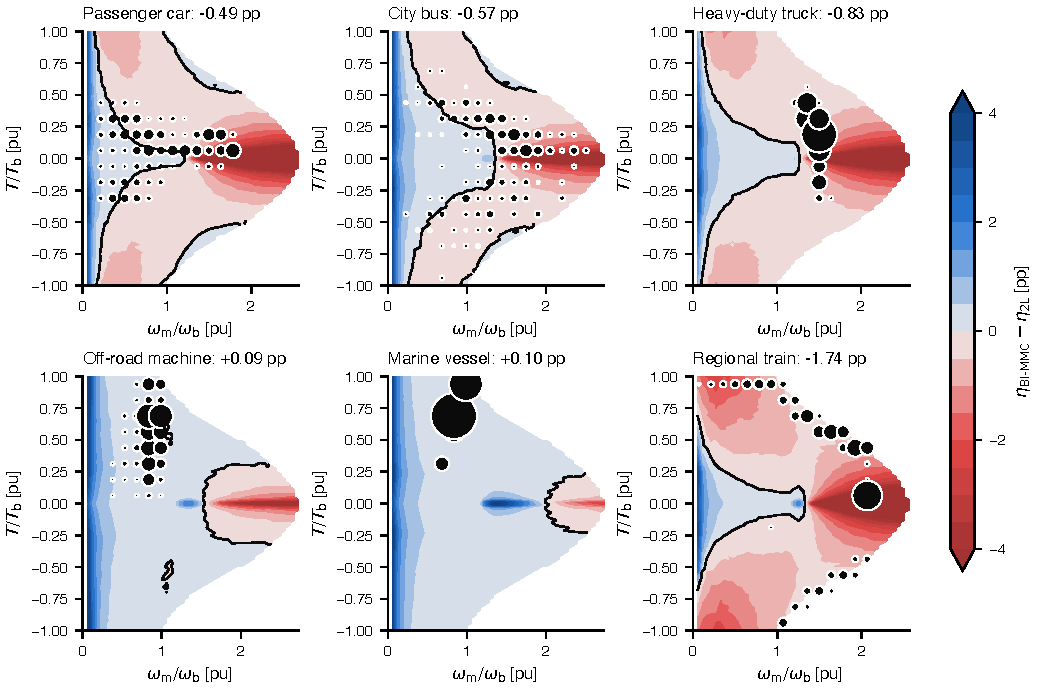
\includegraphics[width=\linewidth]{figures/paper_delta_maps.pdf}
\caption{Efficiency difference BI-MMC $-$ 2L over the torque--speed map at \SI{50}{\percent} SOC for the six applications (colour scale clipped to $\pm4$~pp). Dots: cycle energy $|P|\Delta t$ per bin; dot area is proportional to the energy share. Solid line: $\Delta\eta=0$. The title gives the cycle result $\Delta\etacyc$.}
\label{fig:delta_maps}
\end{figure}

\Cref{tab:ratios} and \cref{fig:summary} summarise the cycle results; \cref{tab:resfull} in the appendix lists the loss energies for all SOC values, and \cref{fig:trace_car,fig:trace_truck} (and the appendix) show the time series.

\begin{table}[ht]
\centering
\caption{Cycle results at \SI{50}{\percent} initial SOC. Semi.\ cut: reduction of semiconductor (conduction + switching) loss energy by the BI-MMC; $E_\mathrm{b}$ ratio: BI-MMC over 2L battery loss energy; $\Delta E_\mathrm{loss}$: relative change of the total loss energy; Cons.: net battery energy per \SI{100}{\kilo\metre} (2L, BI-MMC); $z_\mathrm{end}$: final SOC (2L, BI-MMC).}
\label{tab:ratios}
\footnotesize
\setlength\tabcolsep{4pt}
\begin{tabular}{@{}lrrrrrrr@{}}
\toprule
 & Semi.\ cut & $E_\mathrm{b}$ ratio & $\Delta E_\mathrm{loss}$ & \multicolumn{2}{c}{Cons.\ [kWh/100 km]} & \multicolumn{2}{c}{$z_\mathrm{end}$ [\%]} \\
Application & [\%] & [--] & [\%] & 2L & BI & 2L & BI \\
\midrule
Passenger car & 60 & 4.1 & +43 & 10.6 & 10.7 & 46.8 & 47.0 \\
City bus & 56 & 4.4 & +35 & 50.2 & 51.4 & 48.5 & 48.4 \\
Heavy-duty truck & 37 & 3.0 & +54 & 115.2 & 116.5 & 15.6 & 15.6 \\
Off-road machine & 80 & 1.7 & -9 & -- & -- & 41.4 & 41.5 \\
Marine vessel & 53 & 1.6 & -11 & -- & -- & 24.9 & 25.0 \\
Regional train & 26 & 2.2 & +61 & 165.3 & 170.7 & 38.7 & 38.4
\\
\bottomrule
\end{tabular}
\end{table}

\begin{table}[ht]
\centering
\caption{Cycle efficiency at \SI{50}{\percent} SOC; the second block lists the peak steady-state temperatures along the cycle. $\Delta\etacyc=\etacyc^\mathrm{BI}-\etacyc^\mathrm{2L}$ with the range over \SIrange{20}{90}{\percent} initial SOC.}
\label{tab:etacyc}
\footnotesize
\setlength\tabcolsep{4pt}
\begin{tabular}{@{}lrrrcrrrrrr@{}}
\toprule
 & $\etacyc^\mathrm{2L}$ & $\etacyc^\mathrm{BI}$ & $\Delta\etacyc$ & range & \multicolumn{2}{c}{$\Tj^\mathrm{max}$ [\si{\celsius}]} & \multicolumn{2}{c}{$\Tc^\mathrm{max}$ [\si{\celsius}]} & \multicolumn{2}{c}{$T_\mathrm{cell}^\mathrm{max}$ [\si{\celsius}]} \\
Application & [\%] & [\%] & [pp] & [pp] & 2L & BI & 2L & BI & 2L & BI \\
\midrule
Passenger car & 98.87 & 98.38 & -0.49 & [-0.77, -0.34] & 31 & 25 & 27 & 25 & 25.1 & 25.3 \\
City bus & 98.35 & 97.78 & -0.57 & [-0.86, -0.48] & 50 & 27 & 35 & 25 & 25.2 & 25.3 \\
Heavy-duty truck & 98.45 & 97.62 & -0.83 & [-1.58, -0.48] & 44 & 28 & 32 & 26 & 25.4 & 25.5 \\
Off-road machine & 99.02 & 99.10 & +0.09 & [+0.02, +0.09] & 44 & 25 & 32 & 25 & 25.2 & 25.2 \\
Marine vessel & 99.06 & 99.17 & +0.10 & [+0.05, +0.11] & 48 & 26 & 34 & 25 & 25.0 & 25.1 \\
Regional train & 97.15 & 95.40 & -1.74 & [-2.34, -1.68] & 54 & 29 & 36 & 26 & 26.1 & 26.4
\\
\bottomrule
\end{tabular}
\end{table}

\begin{figure}[ht]
\centering
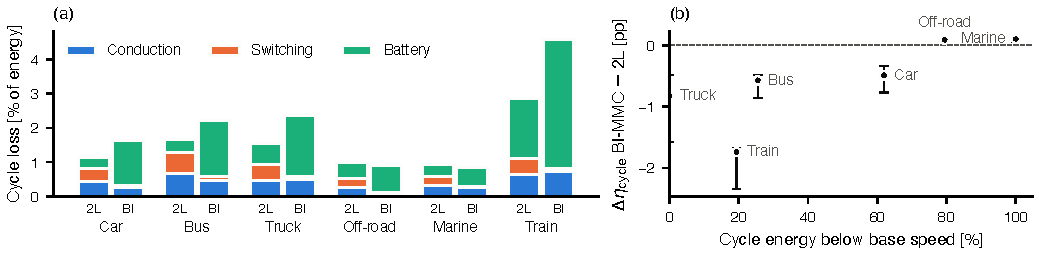
\includegraphics[width=\linewidth]{figures/cycle_summary.pdf}
\caption{(a) Cycle losses by component in percent of the traction energy throughput at \SI{50}{\percent} SOC; (b) cycle efficiency difference BI-MMC $-$ 2L versus the share $\sigma_\mathrm{b}$ of cycle energy below base speed (bars: \SIrange{20}{90}{\percent} SOC).}
\label{fig:summary}
\end{figure}

\paragraph{Where the losses go.} In every application, the BI-MMC cuts the semiconductor loss energy, by \SIrange{37}{80}{\percent} in car, bus, truck, off-road and marine duty and by \SI{26}{\percent} in the train (\cref{tab:ratios}). The saving comes mostly from switching, which almost vanishes (\cref{fig:summary}a). The conduction loss energy of the BI-MMC is lower in car, bus, off-road and marine duty (\SIrange{35}{81}{\percent} of the 2L value) but higher in the truck ($1.04\times$) and the train ($1.13\times$), where the high phase current flows through 11 and 13 series SMs (\cref{tab:resfull}). In exchange the battery loss energy is \numrange{1.6}{4.4} times higher. Because the battery loss is the largest component in all applications, the total loss energy of the BI-MMC is \SIrange{35}{61}{\percent} higher in car, bus, truck and train, and \SIrange{9}{11}{\percent} lower in the off-road machine and the ship. The net battery energy per \SI{100}{\kilo\metre} is correspondingly \SIrange{1.0}{3.3}{\percent} higher for the BI-MMC in the vehicle cycles. The peak junction temperature in the BI-MMC stays within \SI{4}{\kelvin} of the ambient, while the 2L inverter reaches \SIrange{31}{54}{\celsius}; this is a quasi-static estimate that overstates short peaks, and it is far from any limit for both drives.

\paragraph{Cycle efficiency and the share below base speed.} \Cref{fig:summary}b plots $\Delta\etacyc$ against $\sigma_\mathrm{b}$. The BI-MMC gains only when practically all cycle energy is delivered below base speed (marine vessel: $\sigma_\mathrm{b}=\SI{100}{\percent}$, $+0.10$~pp; off-road machine: \SI{79}{\percent}, $+0.09$~pp). Even then the gain is only about \SI{0.1}{\pp}. The truck ($\sigma_\mathrm{b}=0$, $-0.83$~pp) and the train (\SI{19}{\percent}, $-1.74$~pp) operate in field weakening and lose most. The passenger car and the city bus lose \SIrange{0.5}{0.6}{\pp}. The car has \SI{62}{\percent} of its energy below base speed, so $\sigma_\mathrm{b}$ alone is not sufficient: the car's light WLTC loads keep the 2L losses low, so the four-fold battery loss dominates. A low initial SOC lowers the cell voltage, deepens field weakening, and penalises the BI-MMC in all applications except the off-road machine and the ship, where the effect is within \SI{0.1}{\pp} (\cref{fig:soc}). The truck cycle ends at \SI{15.6}{\percent} SOC, so its late part is already in the low-SOC regime.

\begin{figure}[ht]
\centering
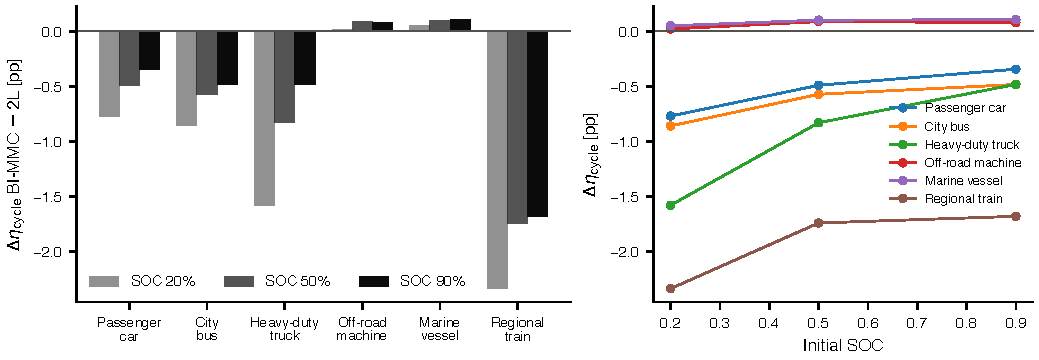
\includegraphics[width=\linewidth]{figures/paper_soc.pdf}
\caption{Cycle efficiency difference BI-MMC $-$ 2L for initial SOC of \SIlist{20;50;90}{\percent}: per application (left) and versus SOC (right).}
\label{fig:soc}
\end{figure}

\begin{figure}[ht]
\centering
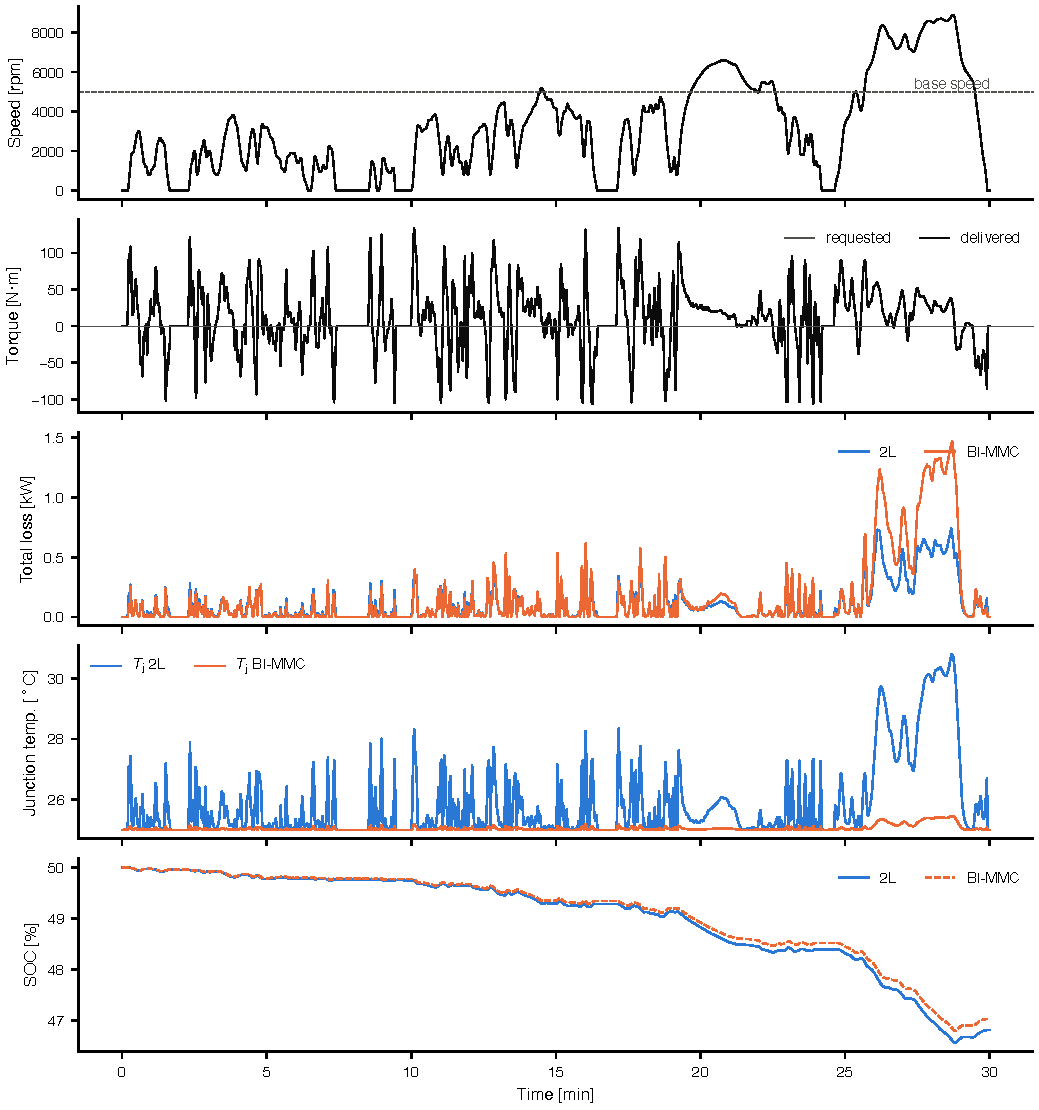
\includegraphics[width=0.9\linewidth]{figures/paper_trace_car.pdf}
\caption{Time series of the passenger car (WLTC, \SI{50}{\percent} initial SOC): machine speed, requested and delivered torque, total loss power, junction temperature, and SOC of both drives.}
\label{fig:trace_car}
\end{figure}

\begin{figure}[ht]
\centering
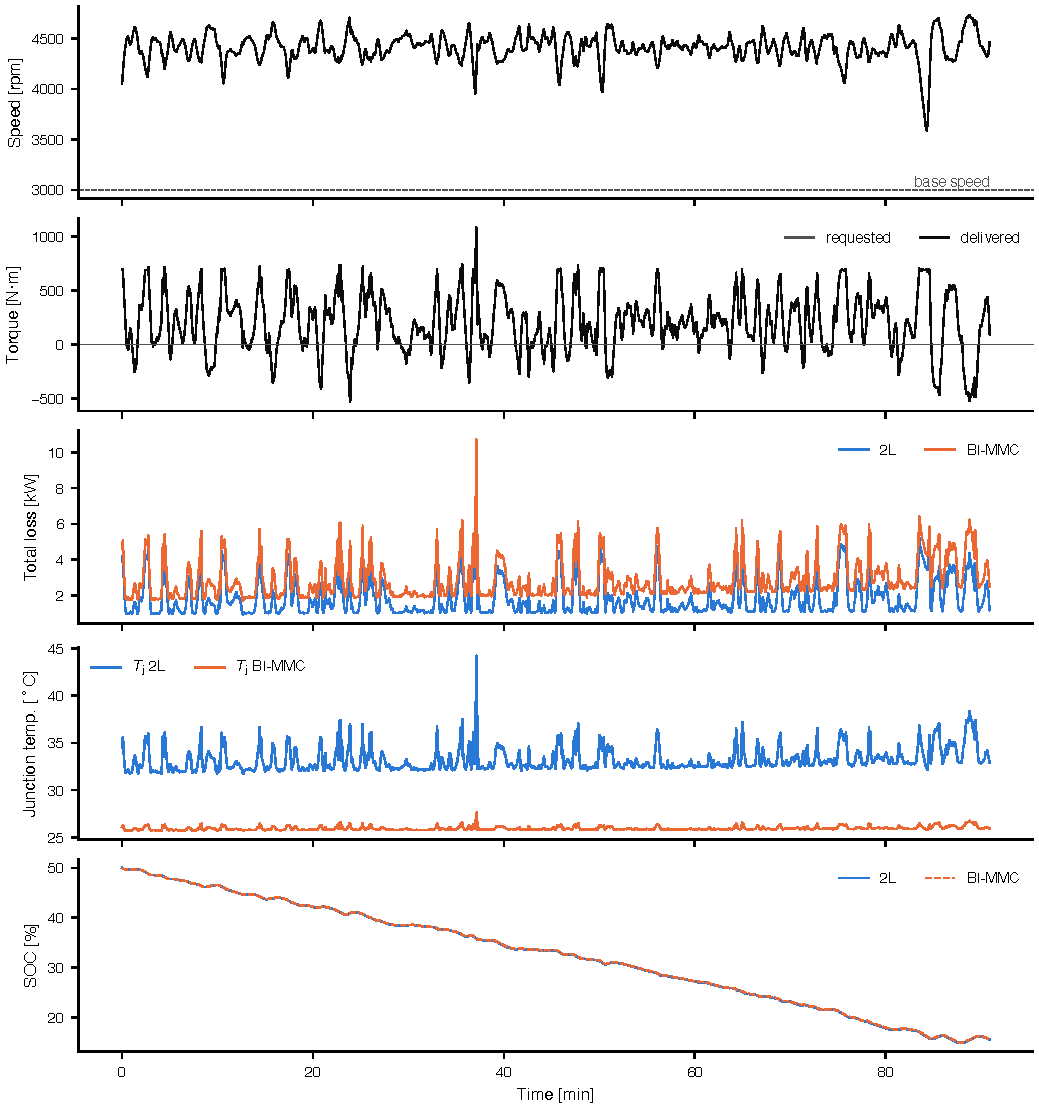
\includegraphics[width=0.9\linewidth]{figures/paper_trace_truck.pdf}
\caption{Time series of the heavy-duty truck (Södertälje--Norrköping, \SI{50}{\percent} initial SOC). The truck stays above base speed on the whole route, which explains the high BI-MMC loss.}
\label{fig:trace_truck}
\end{figure}

\paragraph{Clipped energy.} In the road, off-road and marine cycles, the two drives can deliver the full requested torque (\cref{tab:cycles}). In the synthetic train cycle, the requested regenerative torque (up to \SI{3.8}{\kilo\newton\metre} at the machine) exceeds the base torque of \SI{2.9}{\kilo\newton\metre}, so that the delivered torque differs from the request in \SI{15}{\percent} of the samples, and \SI{11.5}{\kilo\watt\hour} of the \SI{16.1}{\kilo\watt\hour} requested regenerative energy is therefore assigned to the mechanical brake. The train results are thus for a drive that is undersized for the assumed braking, and they should be read with this in mind.
